\section{Application to Montana}

We demonstrate the application of the model at regional scales in the state of Montana, located in the intermountain Pacific northwest of the United States (inset of Figure \ref{fig:hydro_network}). The study region extends beyond the boundaries of the state to include the headwaters of basins that drain into the state, covering an area of 464,800 \si{\kilo\meter\squared}. The state has a longitudinal topographic and climatic gradient, from the steep and relatively wet Rocky mountain western region toward the flatter and significantly drier eastern portions of the state, which are part of the US northern great plains region. The US continental divide runs roughly north to south along the west quarter of the state. About 25\% of  Montana drains to the Pacific (Columbia and Clark Fork basins) and the rest of the state (headwaters of the Missouri basin) is part of the Atlantic basin. Annual precipitation inputs range from over 1000 \si{\milli\meter\per\year} in the mountain regions of the west and gradually decline to about 200 \si{\milli\meter\per\year} in eastern Montana. The western part of the state also shows less continentality, with relatively warmer temperatures in the winter and cooler temperatures in the summer than the eastern portion of the state. 

Other than the ecosystem, the largest water user in the state is agriculture. Agriculture is also a key industry in the state. Despite its economic importance, agriculture is poorly diversified and dominated in terms of production and planted area by alfalfa, wheat, and barley. Montana is a major producer of wheat and barley in the US and contributes to the country's food security. Irrigation is common along streams and in the western parts of the state, however rainfed production is dominant and very vulnerable to drought, especially in the drier central and eastern parts of the state. Irrigation has been growing substantially in the state in recent decades and has contributed to increasing production and reducing economic risk. Surface water is the primary source for irrigation in the west and within irrigation districts, and so far significant groundwater depletion due to agricultural extraction is only limited to a few localized watersheds (\citep[][p. 120]{MCA2017}).

\subsection{Implementation of hydrologic component}

The representation of the hydrologic system in the the study region is shown in Figure \ref{fig:hydro_network}. The figure shows the representative elementary watersheds (REWs) that compose the domain, the nodes that define their outlets, and the links (stream reaches) that connect them. We used the GTOPO30 digital elevation model (DEM) produced by the USGS at 1Km resolution to determine the regional drainage network and partition the domain into REWs using GIS procedures. We used the location of active National Water Information System streamflow gauges as the initial set of nodes to partition the landscape into REWS and then further densified the network with additional nodes until we achieved sufficient spatial detail. The densification was done by allocating nodes in pixels having contributing areas larger than a specified threshold. The minimimum contributing area for a REW was selected such that the total number and sizes of REWS was considered adequate to resolve the spatial variability of streamflows. The final domain contains over 300 REWS with typical sizes around 1400 \si{\kilo\meter\squared}. 

Each REW in the domain has one stream reach with a '\texttt{from\_node}' and '\texttt{to\_node}' attribute that identify the upstream and downstream node of the reach. This information is used to build the network topology and a node adjacency matrix that is used in the the water routing algorithm described in \ref{app:hydrologic_model}. Water diversions occur at 56 selected river nodes, one for each economic unit (county) included in the simulation.  

The model was run with daily gridded precipitation, maximum and minimum air temperatures at a 4\si{\kilo\meter} resolution, automatically retrieved as NetCDF files from the gridMET dataset \citep{Abatzoglou2013}. Temperatures are used internally by the model to calculate reference crop evapotranspiration using the Hargreaves method \citep{Hargreaves1985}.

\subsubsection{Calibration of hydrologic component}

The hydrologic model parameters were calibrated manually against streamflow observations at gauged river nodes and against snow water equivalent observations from the SNOTEL network. All parameters of the HBV rainfall-runoff model and Muskingum-Cunge routing model were adjusted and shared between REWs grouped according to their physiographical (mean elevation, mean slope, area, shape factor) and land use characteristics (fraction of the REW under forest cover and under agriculture) using a standard K-means classification method. In total we calibrated seven groups of parameters corresponding to seven groups of REWs.   

\begin{figure}[t]
    \centering
    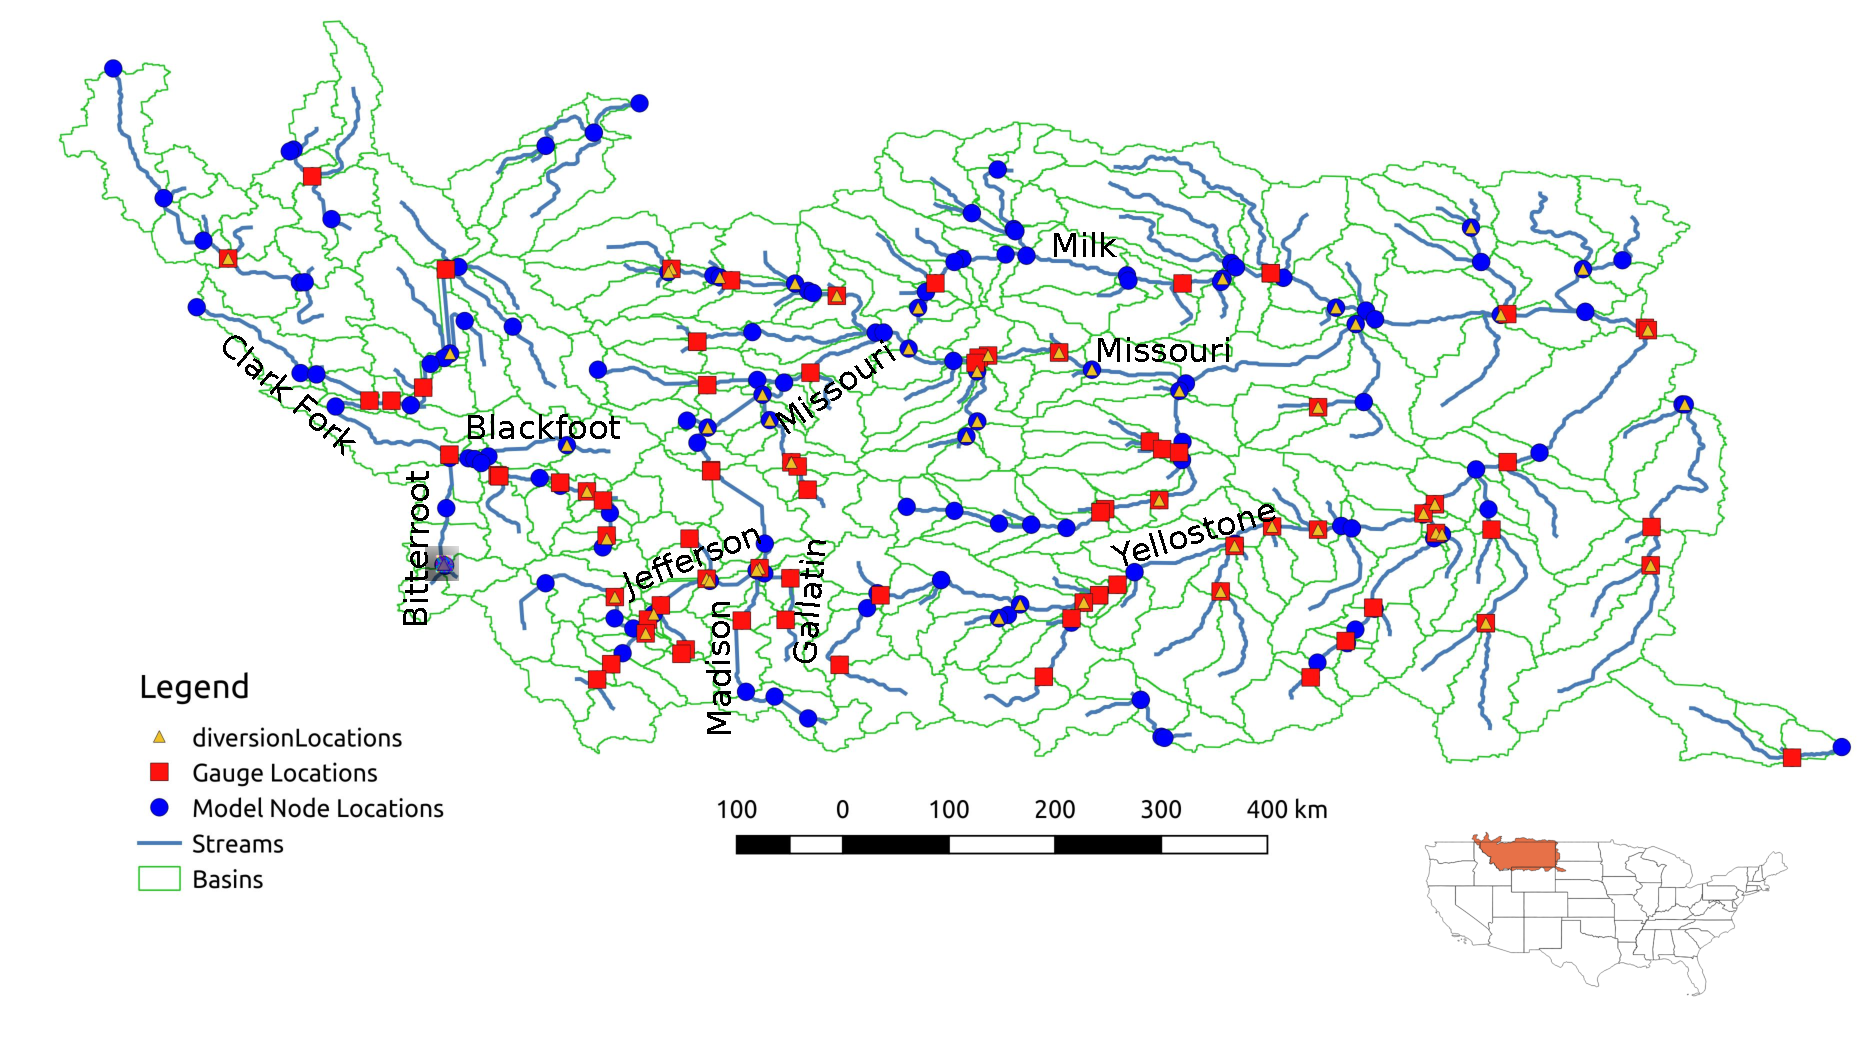
\includegraphics[width=\textwidth]{Figures/HydroNetwork}
    \label{fig:hydro_network}
    \caption{Location of the study region and representation of the hydrologic system and streamflow network}
\end{figure}


\subsection{Implementation of economic component}

Although remote sensing can retrieve information about land and water allocation at field scales, the specification of the economic component of our model is designed to simulate the aggregated economic behavior of producers in a region, not the behavior of individual farms. The economic units considered in this implementation are aggregated at the county level. Thus, we are representing the agricultural system in Montana using 56 economic units (counties), each of them retrieving water from the stream network at one designated diversion node. Although the economic activity is represented in aggregated form, intra-county agroeconomic heterogeneity is, to some extent, implicitly captured in the distribution of model predictions for each county.

\subsubsection{Recursive calibration of the economic component}

Information necessary to update the model parameters include land allocated to each crop, total water used by each crop and total crop production. This information is available every year from remote sensing products at 30 m spatial resolution and then aggregated at county scales. In addition, information on crop prices, approximated variable unit costs of cultivating land and cost of applying water are also required (Table \ref{tab:econ_obs_sources}).

% Please add the following required packages to your document preamble:
% \usepackage{booktabs}
\begin{table}
\caption{Observations necessary to calibrate the economic component}
\centering
\label{tab:econ_obs_sources}
\begin{tabular}{@{}lllll@{}}
\toprule
Observation                    & Units      & Source         & Resolution  \\ \midrule
Land allocation                & ha         & Remote sensing \citep{USDAa} & 30 m, 8 day \\
Water allocation               & mm*ha (decastere)      & Remote Sensing \citep{He2019} & 30 m, 8 day  \\
Crop price                     & \$/ton     & USDA           & State-level, Annual  \\
Cost of land                   & \$/ha      &                & State-level, Annual  \\
Cost of water                  & \$/(mm*ha) &                & State-level, Annual  \\
Crop yield                     & ton        & Remote Sensing \citep{He2018} & 30 m, 8 day   \\
Production elasticity to water & -          & Derived, Eq \eqref{eq:elast_water}        & State-level, Annual  \\
Production elasticity to price & -          & Derived, Eq \eqref{eq:elast_supply}        & State-level, Annual \\ \bottomrule
\end{tabular}
\end{table}

Crop price information and an approximation of production costs were obtained from annual surveys published by the U.S. Department of Agriculture National Agricultural Statistics Service (USDA NASS) at the state scale (QuickStats, \url{http://quickstats.nass.usda.gov}). Crop coefficients to determine crop development stage were obtained from tables published by the AgriMet network for crops grown in the US Pacific Northwest (\url{https://www.usbr.gov/pn/agrimet/cropcurves/crop_curves.html}). 
%Include narrative about data uncertainty. 

Annual variations in crop mix and area are obtained from the USDA Cropland Data Layer, CDL \citep{USDANASS2015}, published by the USDA NASS. The CDL provides a satellite-based, remote sensing annual crop-specific land cover classification that resolves the type and location of the major summer crops in the conterminous US. The CDL is available since 2003 for the conterminous US at 30m spatial resolution. Since the unit of analysis of the economic component is the county, we calculated total allocated land in each county for the main crops grown in Montana (alfalfa, barley  durum wheat, spring wheat, winter wheat, maize and peas) from 2009 to 2018. Uncertainty in land allocation retrievals were estimated by scaling the average pixel level classification uncertainty (standard deviation) of each crop by the number of pixels allocated to the crop in the county. Figure \ref{fig:crop_yield_map}a shows an example of the CDL and the annual variations in allocated area for alfalfa, barley, spring wheat, and winter wheat in two counties. 

\begin{figure}[t]
%\includegraphics[width=0.8\textwidth]{MapsRemoteSensingSamples.pdf}
\includegraphics[width=0.9\textwidth]{Figures/RemoteSensingComposite.png}
\label{fig:crop_yield_map}
\caption{Example of remote sensing retrievals of agricultural activity over the state of Montana. The maps in the figure show pixel-level retrievals in 2009 of a) crop type, location and extent; b) seasonal crop evapotranspiration; and c) crop yield. The time series (insets) show county-aggregated variations of a) total allocated land; b) total county-level crop water use; and c) county-level total production for four example crops (alfalfa, barley, spring wheat and winter wheat) and two example counties (Choteau and Wibaux).  }
\end{figure}

Observations of crop production and yield (defined as the ratio of production to area planted) were obtained using a satellite-driven light use efficiency model to estimate gross primary production (GPP) over croplands at 30 m resolution and 8-day time step. The high spatial and temporal resolution necessary to delineate cropland vegetation growth was achieved by using a NDVI dataset that blended Landsat 5/7 reflectance and Terra MODIS reflectance. Crop yields each year were obtained by accumulating GPP over the growing season and applying a crop-specific harvest index to convert primary production to yields. \citet{He2018} gives a full description and validation of this remote sensing product. We calculated county-scale annual crop production by multiplying crop yield times the area allocated to the crop in each county. Uncertainty in the county-scale production estimates was obtained by scaling the spatial standard deviation of yields by the area planted. Figure \ref{fig:crop_yield_map}c shows an example of the 30m remotely sensed retrieved yield map and the annual variation of alfalfa, barley, spring wheat, and winter wheat production from 2009 to 2018 in two counties. 

Crop water use was estimated by adapting the operational NASA MOD16A2 global ET product \citep{Mu2011}. To better represent cropland ET our adaptation of the MOD16A2 product uses finer scale meteorological inputs from GridMet, and the same refined 30 m resolution NDVI dataset used in the estimation of production. The model parameters were also recalibrated for C3 and C4 crops. A complete description of the adaptation of MOD16A2 ET product for agricultural applications of the Conterminous US is given by \citet{He2019}. Annual variations in county-scale, crop-specific used water volumes were calculated by accumulating pixel-scale ET over the growing season and at the county scale for each crop. Uncertainty in the county-scale water use estimates was obtained by scaling the spatial standard deviation of crop ET by the area planted. Figure \ref{fig:crop_yield_map}b shows an example of the 30m remotely sensed retrieved crop ET map and the annual variation of total water volumes used by alfalfa, barley, spring wheat, and winter wheat production from 2009 to 2018 in two counties. Note that crop water use includes both evapotranspiration from precipitation and from supplemental irrigation. 

\subsection{Analysis methods}

To stabilize the model parameters with the correct values at the beginning of the analysis period we first spun up the data assimilation process by repeatedly ingesting observations from 2008 (first year in our data record) until the posterior distribution of the model parameters converged. This process optimizes the model parameters for the conditions of 2008. After the spin up was complete, we used the resulting model parameters to verify that they correctly reproduce the observed land and water allocation used to calibrate them. After this verification, we started the data assimilation process by sequentially ingesting observations from 2008 to 2016. Observations from 2017 and 2018 were available but not ingested and used to verify the the ability of the model to predict out of sample years. The model verification and analysis focused mostly on the predictions of land and water allocation, since it is one of the most novel aspect of the modeling system. However, we also demonstrated the value added by the hydrologic component by identifying the net impact of agricultural water diversions in 2017. The spatial impacts of agricultural water use were discussed qualitatively.     


